\documentclass{ximera}
%% handout
%% nohints
%% space
%% newpage
%% numbers

\input{preamble.tex} %% we can turn off input when making a master document

\outcome{Understand a first example of the Ximera style.}
\outcome{Have a nice basic example to work from.}
\outcome{See if all of this works with English Grammar}

\title{First Example for English Grammar}

\begin{document}
\begin{abstract}
In this activity we see some examples of English grammar questions.
\end{abstract}
\maketitle

To start, watch this video:

VIDEO:

\youtube{http://www.youtube.com/watch?v=8BFsz1FCdxM}


\begin{exercise}
What verb tense did the speaker use most frequently?

\begin{solution}

\begin{hint}
Everything she described happened yesterday.
\end{hint}
\begin{hint}
Yesterday is in the past.
\end{hint}
What verb tense did the speaker use most frequently? \answer{past}.
YYY
\end{solution}
\end{exercise}



\begin{question}
In the following sentence, what verb tense is used?
Helen went to the store yesterday.

\begin{solution}
\begin{multiple-choice}
\choice{simple present}
\choice[correct]{simple past}
\choice{simple future}
\choice{present perfect}
\choice{past progressive}
\end{multiple-choice}
\begin{hint}
Helen did this yesterday
\end{hint}
\begin{hint}
Yesterday is in the past.
\end{hint}
\end{solution}
\end{question}

\begin{question}



\begin{shuffle}
\begin{question}
In the plot below, is $P$ a function of $k$?
\begin{image}
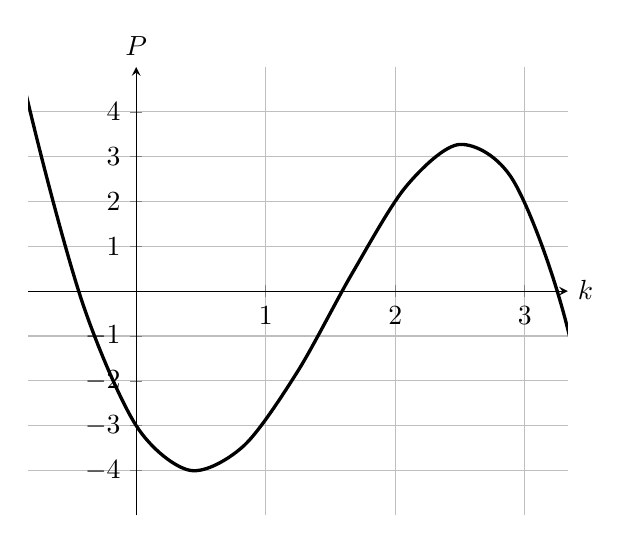
\begin{tikzpicture}
\begin{axis}[
            ymin=-5,
			ymax=5,
            axis lines =center, xlabel=$k$, ylabel=$P$,
              every axis y label/.style={at=(current axis.above origin),anchor=south},
              every axis x label/.style={at=(current axis.right of origin),anchor=west},
            domain=-5:5,
            grid = major,
            xtick={-4,...,4},
            ytick={-4,...,4},
          ]
          \addplot [very thick, smooth] {1 + (3.5 + x)*(-0.5714285714285714 + (-3.5 + x)*(0.16326530612244897 + (-0.3327149041434756 + (-0.20522334808049095 + 0.04019472590901159*(-3 + x))*(-2 + x))*x))};
        \end{axis}
\end{tikzpicture}
\end{image}
\begin{solution}
\begin{multiple-choice}
\choice[correct]{Yes.}
\choice{No.}
\end{multiple-choice}
\begin{hint}
For each input, how many outputs are there?
\end{hint}
\end{solution}
Use the plot to compute $P(2)$.
\begin{solution}
\begin{hint}
To start, find $2$ on the horizontal axis. 
\end{hint}
\begin{hint}
Now from this position, move up or down until you reach the curve. The value of $P(2)$ is the height of the curve at the point $k=2$.
\end{hint}
The value of $P(2)$ is \answer{$2$}.
\end{solution}
\end{question}


\begin{question}
In the plot below, is $R$ a function of $n$?
\begin{image}
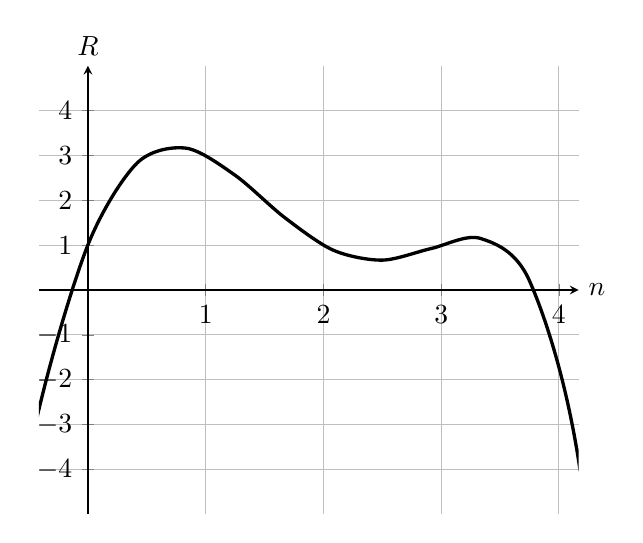
\begin{tikzpicture}
\begin{axis}[
            ymin=-5,
			ymax=5,
            axis lines =center, xlabel=$n$, ylabel=$R$,
              every axis y label/.style={at=(current axis.above origin),anchor=south},
              every axis x label/.style={at=(current axis.right of origin),anchor=west},
            domain=-5:5,
            grid = major,
            xtick={-4,...,4},
            ytick={-4,...,4},
          ]
          \addplot [very thick, smooth] {4 + (-0.42857142857142855 + (-0.05952380952380952 + (0.09163059163059163 + (-0.041447441447441453 - 0.08955488955488956*(-3 + x))*(-2 + x))*(-0.5 + x))*(-3.5 + x))*(3.5 + x)};
        \end{axis}
\end{tikzpicture}
\end{image}
\begin{solution}
\begin{multiple-choice}
\choice[correct]{Yes.}
\choice{No.}
\end{multiple-choice}
\begin{hint}
For each input, how many outputs are there?
\end{hint}
\end{solution}
Use the plot to compute $R(3)$.
\begin{solution}
\begin{hint}
To start, find $3$ on the horizontal axis. 
\end{hint}
\begin{hint}
Now from this position, move up or down until you reach the curve. The value of $R(3)$ is the height of the curve at the point $n=3$.
\end{hint}
The value of $R(3)$ is \answer{$1$}.
\end{solution}
\end{question}

\begin{question}
In the plot below, is $b$ a function of $w$?
\begin{image}
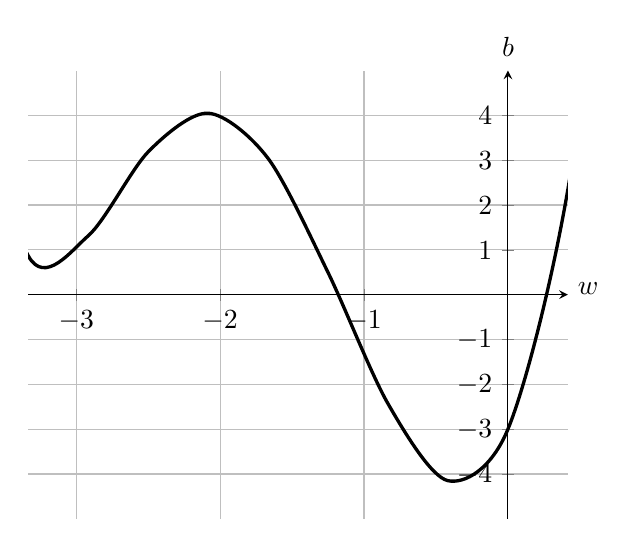
\begin{tikzpicture}
\begin{axis}[
            ymin=-5,
			ymax=5,
            axis lines =center, xlabel=$w$, ylabel=$b$,
              every axis y label/.style={at=(current axis.above origin),anchor=south},
              every axis x label/.style={at=(current axis.right of origin),anchor=west},
            domain=-5:5,
            grid = major,
            xtick={-4,...,4},
            ytick={-4,...,4},
          ]
          \addplot [very thick, smooth] {2 + (3.5 + x)*(0.2857142857142857 + (-3.5 + x)*(0.489795918367347 + x*(0.34013605442176864 + (-0.5850340136054422 - 0.25117739403453676*(-0.5 + x))*(2 + x))))};
        \end{axis}
\end{tikzpicture}
\end{image}
\begin{solution}
\begin{multiple-choice}
\choice[correct]{Yes.}
\choice{No.}
\end{multiple-choice}
\begin{hint}
For each input, how many outputs are there?
\end{hint}
\end{solution}
Use the plot to compute $b(-2)$.
\begin{solution}
\begin{hint}
To start, find $-2$ on the horizontal axis. 
\end{hint}
\begin{hint}
Now from this position, move up or down until you reach the curve. The value of $b(-2)$ is the height of the curve at the point $w=-2$.
\end{hint}
The value of $b(-2)$ is \answer{$4$}.
\end{solution}
\end{question}
\end{shuffle}



\end{document}
